% main.tex -- QVLA, submitted to MIDI 2026 (Springer LNNS proceedings, LNCS layout)
% Compile: pdflatex -> bibtex -> pdflatex -> pdflatex   (Overleaf: default pdfLaTeX)
% Page limit: 8 pages including references (MIDI 2026 call for papers).
\documentclass[runningheads]{llncs}
%
\usepackage[T1]{fontenc}
\usepackage{newtxtext}
\usepackage[varvw]{newtxmath}
\usepackage{graphicx}
\usepackage{color}
\usepackage{hyperref}
\hypersetup{hidelinks}   % no link boxes; URLs stay blue via \UrlFont (Springer eBook style)
\renewcommand\UrlFont{\color{blue}\rmfamily}
\urlstyle{rm}
%
\begin{document}
%
\title{QVLA: Training-Free Language-Driven Robot Navigation by Choosing Among Arcs Drawn on the Camera Image}
\titlerunning{QVLA: Choosing Among Arcs Drawn on the Camera Image}
%
% Optional: ORCID iDs, e.g. \author{Fouad Aladhami\orcidID{0000-0000-0000-0000} \and ...}
\author{Fouad Aladhami\inst{1} \and Ozan Berk Kaya\inst{1} \and Salih Sarp\inst{2}}
\authorrunning{F. Aladhami et al.}
\institute{Department of Computer Engineering, Gebze Technical University, Kocaeli, T\"urkiye\\
\email{f.aladhami2021@gmail.com}, \email{o.kaya2025@gtu.edu.tr}
\and
Department of Data Science and Analytics, Gebze Technical University, Kocaeli, T\"urkiye\\
\email{salih@gtu.edu.tr}}
%
\maketitle
%
\begin{abstract}
Navigation vision-language-action (VLA) policies map camera frames and an instruction to
waypoints, but a recent one barely listens: swapping ``turn left'' for ``turn right'' moves
its planned heading by 0.04--36$^\circ$, while changing the scene moves it by 53$^\circ$.
We present QVLA, a training-free policy in which a frozen vision-language model
(Qwen3.8-27B) never writes a coordinate. Seven arcs of known curvature are drawn on the camera
image under shuffled labels; the model first describes the scene (what blocks the way, which
side is open, how far the goal is), then answers with one label, which a plan builder, a
pure-pursuit controller and a collision guard turn into motion. Its instruction moves the plan
by 102$^\circ$, and asking it first to name the open side raises wall avoidance from 22\% to
100\% of blocked frames. On the DynaNav benchmark in Isaac Sim, on a mobile manipulator that
neither method was designed for, every policy ran three times on identical code. QVLA reached
7.7 of 13 indoor goals per round and TIC-VLA, fine-tuned on DynaNav, 6.3: a difference within
run-to-run variation (paired sign-flip $p=0.69$). A baseline without a model, which always
takes the straight arc, reached 1. The two policies fail differently: QVLA ends far from the
goal after missing a turn toward a goal it cannot yet see, TIC-VLA within a few metres of it.
We report variance, ablations and failure modes.

\keywords{Vision-language models \and Robot navigation \and Zero-shot learning \and
Visual prompting \and Vision-language-action models.}
\end{abstract}
%
%
\section{Introduction}
\label{sec:intro}

Language-driven navigation asks a robot to carry out a sentence such as ``go straight ahead
and stop at the nearest elevator'' from its own camera. The current trend is to fine-tune a
vision-language model (VLM) on instruction-paired trajectories so that it emits waypoints or
actions~\cite{brohan2023rt2,kim2024openvla,zhang2024navid}. TIC-VLA~\cite{huang2026ticvla}
does so for dynamic scenes: a slow VLM reasons in text and fills a key-value cache that a fast
action expert reads to produce waypoints; its DynaNav benchmark runs in Isaac Sim~\cite{isaacsim}.
Porting TIC-VLA to another robot, we found its plans governed by the scene rather than the
sentence (Sect.~\ref{sec:authority}). A frozen general-purpose VLM has the opposite profile:
it follows words but emits poor coordinates. Asked for ten waypoints, Qwen3.8-27B~\cite{qwen38} wrote the same straight
line, lateral offset exactly 0.00, for five unrelated scenes, even after its own reasoning had
concluded that it should move ``forward and left''.

QVLA keeps the VLM for what it does well---reading an image and a sentence---and takes the
geometry out of its answer: candidate paths are drawn on the image and the model names one.
We contribute (i)~a training-free policy around a frozen 27B VLM: an arc menu with shuffled
labels, a describe-then-select chain, a speed channel and recovery, executed asynchronously
by a conventional controller; (ii)~a closed-loop DynaNav evaluation on a mobile manipulator
against TIC-VLA and a baseline without a model, on identical infrastructure with three
interleaved runs each, with its biases stated; and (iii)~probes that
separate instruction following from free-space perception with label-free mirror
controls.\footnote{Code, configurations and per-run logs:
\url{https://github.com/GTU-DASH-LAB/dash-aloha-mini-isaacsim/tree/midi2026}}

\section{Related Work}
\label{sec:related}

Zero-shot object navigation systems such as CoWs~\cite{gadre2023cows},
VLFM~\cite{yokoyama2024vlfm} and WMNav~\cite{nie2025wmnav} score frontiers or objects on a map
with a foundation model and reach them with a classical planner, relying on depth and mapping;
QVLA uses one RGB camera and no map, and the model's choice is itself the local plan.
Vision-and-language navigation~\cite{anderson2018vision} has been approached by composing
pretrained models, as in LM-Nav~\cite{shah2022lm}, and by fine-tuning VLMs to emit motions or
action tokens~\cite{brohan2023rt2,huang2026ticvla,kim2024openvla,zhang2024navid}. Closest to QVLA is
visual prompting: Set-of-Mark~\cite{yang2023som} labels image regions for a VLM to refer to,
PIVOT~\cite{nasiriany2024pivot} iteratively samples arrows drawn on the image, and
VLMnav~\cite{goetting2024vlmnav} draws discrete navigation actions using depth. QVLA is
built from these known parts, and its contribution is in how they are joined and in what we
measure. The drawn arcs are exactly the plans the controller executes, so what the model
picks is what the robot does. Labels are reshuffled at every decision, so a positional habit
scores at chance. Perception and choice are split into two calls, the first of which names
the open side; together these raise wall avoidance on blocked frames from 22\% to 100\%
(Sect.~\ref{sec:freespace}).
We also separate instruction following from scene following with matched controls, for
QVLA and for a fine-tuned navigation VLA.

\section{Method}
\label{sec:method}

\begin{figure}[t]
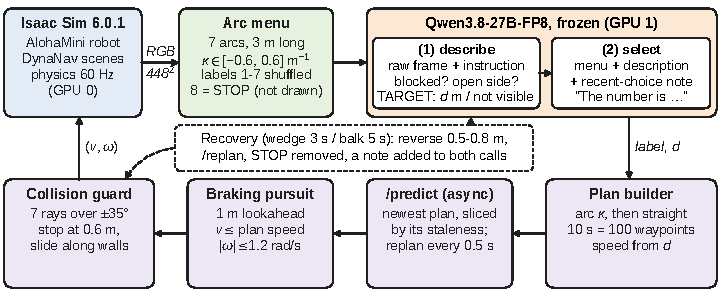
\includegraphics{figures/fig1_overview.pdf}
\Description{Block diagram of QVLA. Top row: Isaac Sim sends a 448 by 448 RGB frame to the arc
menu, which draws seven arcs with shuffled labels; a frozen Qwen3.8-27B model first describes
the raw frame and then selects a label from the menu image. Bottom row, right to left: the
label and a distance estimate go to a plan builder, an asynchronous predict endpoint, a braking
pure-pursuit controller and a collision guard, which sends linear and angular velocity back to
the simulator. A dashed recovery box connects the guard back to the model.}
\caption{QVLA. Top: perception and decision, about one decision per 2.1\,s. Bottom:
execution, replanned every 0.5\,s and tracked at 60\,Hz. Only the dashed recovery path
reverses the robot.}
\label{fig:overview}
\end{figure}

Fig.~\ref{fig:overview} shows the two loops. A decision loop runs the VLM on the newest frame
whenever it is free. A control loop posts the frame and robot state to an asynchronous
\texttt{/predict} endpoint every 0.5\,s of simulated time and receives the newest plan minus
its first $\lceil\tau/\Delta t\rceil$ waypoints, $\tau$ being the plan's age.

\subsection{Arc Menu}
\label{sec:menu}

The menu has seven arcs with curvatures $\kappa\in\{0,\pm0.15,\pm0.35,\pm0.60\}\,\mathrm{m^{-1}}$
and length $L=3$\,m. In the robot frame ($x$ forward, $y$ left) the point at arc length $s$ is
\begin{equation}
x(s)=\frac{\sin(\kappa s)}{\kappa},\qquad y(s)=\frac{1-\cos(\kappa s)}{\kappa},
\label{eq:arc}
\end{equation}
with the straight line as the limit $\kappa\to0$. Each point is projected with the pinhole
model of a level camera mounted $h$ above the floor,
\begin{equation}
u=\frac{W}{2}-f\,\frac{y}{x},\qquad v=\frac{H}{2}+f\,\frac{h}{x},\qquad
f=\frac{W/2}{\tan(\phi/2)},
\label{eq:proj}
\end{equation}
where $\phi$ is the horizontal field of view. The camera copies the one DynaNav's robot is
trained with ($\phi=90.1^\circ$, $h=0.346$\,m, $1920\times1080$), since a VLA's camera is part
of its input distribution; frames are downscaled to $448\times448$. Each arc ends in a
numbered circle; labels 1--7 are a fresh random permutation at every decision, so any
positional habit scores at chance. Label 8 (STOP) is not drawn
(Figs.~\ref{fig:menu}a and~\ref{fig:qual}).

\begin{figure}[t]
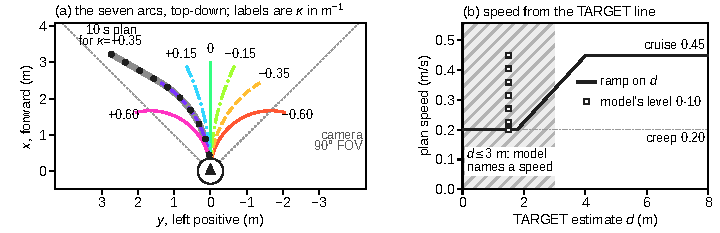
\includegraphics{figures/fig2_menu.pdf}
\Description{Two panels. Left: top-down view of the seven arcs fanning out from the robot
with curvature labels from minus 0.60 to plus 0.60, the dotted edges of the 90 degree camera
field of view, and a grey 10 second plan for curvature plus 0.35 that follows the arc for
3 metres and then continues straight, with a dot every second. Right: plan speed against the
TARGET distance estimate, a ramp from 0.20 metres per second below 1.8 metres to 0.45 above
4 metres; a hatched region below 3 metres where the model also names a speed level, shown as
squares between 0.20 and 0.45.}
\caption{(a)~The seven arcs in the robot frame, and the 10\,s plan that label
$\kappa=+0.35$ becomes at 0.45\,m/s (one dot per second). (b)~Plan speed against the model's
TARGET estimate $d$; inside 3\,m the model also names a speed level $\ell$.}
\label{fig:menu}
\end{figure}

\subsection{Describe, Then Select}
\label{sec:chain}

Each decision makes two calls to the same frozen model. \emph{Describe} sees the raw frame
and answers in at most 110 tokens: whether a wall, door or large object is straight ahead
within about 3\,m; which direction has the most open floor (\emph{far left, left, straight
ahead, right, far right}); and a final line \texttt{TARGET:~<n>~m} or
\texttt{TARGET:~not~visible} for the place the instruction names. \emph{Select} sees the menu image, the instruction, the description and a one-line history of
recent choices, with one rule: \emph{``The instruction may list several moves in order; do
only the earliest one not yet done. Where it names a direction the description does not call
open, follow the description.''} STOP is allowed only on arrival or when every path is
blocked. The reply is prefilled with ``The number is'' and decoded greedily for at most 8
tokens; nothing is trained.

\subsection{From a Label to Motion}
\label{sec:plan}

The plan follows the chosen arc for 3\,m and then its final heading, sampled at
$\Delta t=0.1$\,s over 10\,s (Fig.~\ref{fig:menu}a); longer turns come from choosing a curved
arc again. The horizon must outlast a generation: with TIC-VLA's 3\,s horizon, slicing a plan by
its own age left at most one waypoint, and an early version stood still on 129 of 141 calls. Speed follows the TARGET line (Fig.~\ref{fig:menu}b):
$v=\min(0.45,\max(0.20,\,0.45\,d/4))$\,m/s, or 0.45\,m/s if the target is not visible; within
3\,m the select call also names a level $\ell\in\{0,\dots,10\}$ and
$v=\min(0.45,\max(0.20,\,0.045\,\ell))$.

A braking pure-pursuit controller~\cite{coulter1992pure} never exceeds the plan's speed. The
simulated wheels lack traction, so the base is driven kinematically. A contact layer sweeps
the robot's collision envelope (base, lift and arms) along every step and stops it 2\,cm short
of anything it would hit, keeping the motion along the surface, so no policy can drive through
an obstacle; steps up to 4.5\,cm are climbed. A guard casts 7 rays over $\pm35^\circ$ around the
direction of travel and removes the velocity component pointing into any obstacle within
0.6\,m, so the robot slides along walls rather than freezing. A \emph{wedge} (under 0.1\,m of progress in 3\,s, obstacle ahead)
reverses up to 0.8\,m; a \emph{balk} (stationary for 5\,s, front clear) reverses 0.5\,m.
Recovery also discards the cached plan, removes STOP from the next decision and tells both
prompts that the robot has just reversed.

\section{Experimental Setup}
\label{sec:setup}

Isaac Sim 6.0.1~\cite{isaacsim} runs physics at 60\,Hz on one 32\,GB GPU and the FP8 VLM
(28.75\,GiB) on a second. The robot is AlohaMini~\cite{alohamini}, a three-wheel
omnidirectional base with a lift and two arms (held still).
DynaNav~\cite{huang2026ticvla} defines 85 episodes in hospital, office, warehouse and outdoor
scenes; its published reference run of TIC-VLA on its own robot covers 49 and completes 29.
Our indoor set takes the 11 of those 29 easiest for our robot by turn size, detour and length,
so the reference run succeeds on all 11 (mean SPL 0.98) and the selection favours the
baseline. We add two unscored warehouse episodes, for 13; every start heading is within
about 30$^\circ$ of the goal bearing. We leave out DynaNav's outdoor scene: our early runs
there were affected by simulation defects that we have since fixed, and after the fixes its
failures are dominated by kerbs higher than our robot can climb, which measures the robot
rather than the policy.

Three policies run on the same code, robot, camera, controller, guard, contact layer and
recovery reverse. TIC-VLA (InternVL3-1B plus action expert, official checkpoint) runs
asynchronously as in DynaNav, with its four-frame history and waypoint-history text. QVLA's
recovery also discards its plan and notes the reverse in its prompts; this part does not
apply to TIC-VLA. A no-model baseline takes the straight arc at cruise speed at every
decision and shows how much of the task needs no decision at all. Each policy runs the 13
episodes three times, in interleaved rounds (each round runs all three in turn), so that any
slow drift in the machine affects every policy alike; one episode whose scene failed to
load was re-run. Success means coming within 1.5\,m of the goal, which latches. We report success rate (SR) per round,
SPL~\cite{anderson2018evaluation}, mean closest approach, guard interventions (control steps
in which the guard altered the command) and DynaNav's physical-collision flag (contact held
for 3.3\,s). Policies are compared per episode: each episode's success rate over the three
rounds, paired across policies, with an exact sign-flip test and a bootstrap interval over
episodes.

\section{Results}
\label{sec:results}

\subsection{Authority of the Instruction}
\label{sec:authority}

\begin{figure}[t]
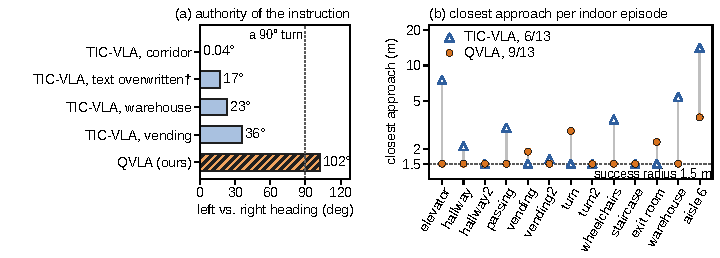
\includegraphics{figures/fig3_results.pdf}
\Description{Two panels. Left: horizontal bars of the heading difference between turn left and
turn right instructions: TIC-VLA corridor 0.04 degrees, TIC-VLA with its reasoning text
overwritten 17 degrees, TIC-VLA warehouse 23 degrees, TIC-VLA vending 36 degrees, and QVLA
102 degrees, beyond a dashed line at a 90 degree turn. Right: for each of the 13 indoor
episodes, the number of successes in three rounds for TIC-VLA (triangles), QVLA (circles) and
a baseline without a model (squares). QVLA succeeds in all three rounds on the elevator, both
down-the-hallway and both vending-machine episodes; TIC-VLA on the wheelchair, staircase and
exit-room episodes; the baseline only on the elevator episode.}
\caption{(a)~Heading difference between ``turn left'' and ``turn right'' on otherwise
identical inputs. TIC-VLA: planned heading in three scenes; $\dagger$~reasoning text
overwritten with explicit left/right text and offsets. QVLA: end-point bearing of the chosen
3\,m arcs, 144 trials. (b)~Successes per indoor episode in three interleaved rounds on
identical code; the legend gives each policy's mean successes per round.}
\label{fig:results}
\end{figure}

Over 144 rendered decisions with ``turn left'', ``turn right'' and ``go straight'', QVLA chose
an arc on the correct side in 100\% of trials for each instruction (random: 43\%); its mean
left and right curvatures differ by 1.19\,m$^{-1}$, 99\% of the menu's span or 102$^\circ$ of
end-point bearing (Fig.~\ref{fig:results}a). With frame, history and state fixed, the same
swap moved TIC-VLA by 0.04$^\circ$ in a corridor, 23.4$^\circ$ at a warehouse start and
35.6$^\circ$ near a vending machine, whereas changing the scene under a fixed instruction
moved it by 52.95$^\circ$ (s.d., eight scenes). Overwriting its reasoning text with explicit
left/right statements and offsets separated the plans by 17.2$^\circ$, of which the words give
about 2$^\circ$ (a cooking recipe containing a large offset gave 15.0$^\circ$), consistent
with training instructions written after the fact from the trajectory.

\subsection{Seeing Free Space}
\label{sec:freespace}

Told only ``Drive safely'', a selector asked for a bare label drove the straight arc into the
wall on 89\% of blocked frames, and never flipped its choice when the frame was mirrored
(0/18). Yet asked which of a blocked and an open frame was open, the model was right 70 of 70
times, and it named the obstacle on 6 of 6 blocked frames: the failure was in the question.
Table~\ref{tab:probe} compares four ways of asking on identical frames and labels.
\emph{Avoid}: blocked frames on which a curved arc was chosen; \emph{keep}: open corridors on
which the straight arc was kept, which catches a policy that merely swerves; \emph{side}: turns
towards the hand-labelled open side (chance 43\%); \emph{mirror}: pairs whose curvature flips
sign under mirroring, which needs no labels. Reasoning in the same call (THINK) helps
little; CHAIN's description says the way is blocked but not which way is open, so the second
call guesses. Asking the first call to \emph{name} the open side (SIDED) is the only variant
above chance on all four columns, at 2.1\,s per decision instead of 0.31\,s. Smaller models
lose most of the side and mirror signal.

\begin{table}[t]
\caption{Open-loop obstacle probe (\%). Set A: 12 frames (6 blocked, 6 open), each also
mirrored, 3 label shuffles. Set B: a harder, later set, not comparable with A. Latency:
median per decision.}
\label{tab:probe}
\centering
\begin{tabular}{llccccc}
\hline
Set & Variant (model) & Avoid & Keep & Side & Mirror & Latency \\
\hline
A & DIGIT: bare label, one call (27B)             & 22  & 100 & 20 & 0  & 0.31\,s \\
A & THINK: reason, then label, one call (27B)     & 33  & 86  & 37 & 17 & 2.42\,s \\
A & CHAIN: describe, then select (27B)            & 72  & 100 & 60 & 28 & 2.10\,s \\
A & SIDED: CHAIN + \emph{name open side} (27B)    & \textbf{100} & 92 & \textbf{90} & \textbf{83} & 2.10\,s \\
\hline
B & DIGIT (27B)                                   & 8   & 100 & 25 & 0  & 0.32\,s \\
B & SIDED (27B)                                   & \textbf{67} & \textbf{100} & \textbf{69} & \textbf{50} & 2.30\,s \\
B & SIDED (Qwen3-VL-4B)                           & 22  & 94  & 36 & 22 & 0.41\,s \\
\hline
\end{tabular}
\end{table}

\subsection{Closed-Loop Navigation}
\label{sec:closed}

\begin{table}[t]
\caption{Closed loop on DynaNav, 13 indoor episodes, three interleaved rounds per policy on
identical code (mean $\pm$ s.d.\ over rounds; range in brackets). Closest: closest approach,
mean over runs (median). Guard: interventions per round of 13 episodes. Coll.: DynaNav
physical collisions per round. DN-11: the 11 episodes DynaNav scores. First row: TIC-VLA on
its own robot, as published by DynaNav.}
\label{tab:closed}
\centering
\begin{tabular}{lcccccc}
\hline
Policy & Success (of 13) & SPL & Closest (m) & Guard & Coll. & DN-11 SR (SPL) \\
\hline
\emph{TIC-VLA, reference run} & -- & -- & -- & -- & -- & \emph{11/11 (0.98)} \\
No model (straight arc) & 1.0 $\pm$ 0.0 [1--1] & 0.08 & 7.33 (3.50) & 10511 & 4.0 & 1.0/11 (0.09) \\
TIC-VLA (fine-tuned 1B) & 6.3 $\pm$ 0.6 [6--7] & 0.47 & \textbf{2.80} (1.54) & \textbf{852} & \textbf{0.7} & 6.0/11 (0.53) \\
QVLA (frozen 27B)       & \textbf{7.7} $\pm$ 1.2 [7--9] & \textbf{0.57} & 4.92 (\textbf{1.50}) & 1562 & 1.7 & \textbf{7.3}/11 (\textbf{0.64}) \\
\hline
\end{tabular}
\end{table}

Every policy ran the 13 indoor episodes three times on the same code (Table~\ref{tab:closed},
Fig.~\ref{fig:results}b). QVLA succeeded on 7.7 episodes per round (7, 7, 9) and TIC-VLA on
6.3 (6, 6, 7). Per episode QVLA did better on 7 and worse on 4, but the mean difference,
+0.10 successes per episode (95\% bootstrap interval $-0.26$ to $+0.46$), is not significant
(exact sign-flip test over episodes, $p=0.69$). Both are far above the baseline without a
model, which shares the menu, controller, guard and recovery but always takes the straight
arc: it succeeds only on the episode whose instruction is to go straight ($p=0.004$ against
QVLA, $p=0.041$ against TIC-VLA). The controller and guard do not reach the goals by
themselves; the choices do.

The two policies succeed on different episodes. QVLA succeeded in all three rounds on the
elevator and both vending-machine episodes, where the sentence decides the route; TIC-VLA solved
them 0, 1 and 0 times out of three. TIC-VLA succeeded in all three rounds on the wheelchair,
staircase and exit-room episodes, which need a turn toward a goal that is not yet in view;
QVLA solved them 0, 0 and 1 times. These misses are why QVLA's mean closest approach is the
larger, 4.9 against 2.8\,m, while the medians are equal: its failures end 9.8\,m from the goal
on average, TIC-VLA's 4.1\,m. Its higher guard count comes from the same hard episodes. Both
policies pressed into an office security desk at the height of the robot's lift carriage, which
the guard's 0.3\,m plane passes under; QVLA also pressed into floor clutter in a warehouse
aisle.

Two caveats bound the comparison. TIC-VLA's model is 27 times smaller, by design, since its
action expert runs at control rate; and model size matters for QVLA, which on an earlier
version of our stack fell from 6--9 to 3 of 13 indoor goals with Qwen3-VL-4B, as its drop in
open-loop wall avoidance (67\% to 22\%, Table~\ref{tab:probe}) predicted. And both policies run
on a robot TIC-VLA was not trained on: on its own robot DynaNav reports 11/11 on this subset.

\paragraph{Ablations and variance.} The menu was tuned on an earlier version of our
simulation stack, against same-study references. Thinking budgets of 180--420 tokens in the
select call scored 2/13 and 2/13 against 7/13; eleven finer arcs with in-place turns 2/18
against 9/18; the previous menu frame as memory 3/19 against 10/19; and a lidar clearance
filter on the arcs 10/19 against 10/19. The simplest menu was the best we found. Seven
repeats of it on that stack scored 6--9 of 13 (mean 7.7), the same mean as here. Despite
greedy decoding and identical labels, repeated runs diverge: the first rendered frame already
differs by about one grey level, the description changes first, and the choice follows 5--20
decisions later.

\subsection{Qualitative Behaviour and Failure Analysis}
\label{sec:qual}

\begin{figure}[t]
\centering
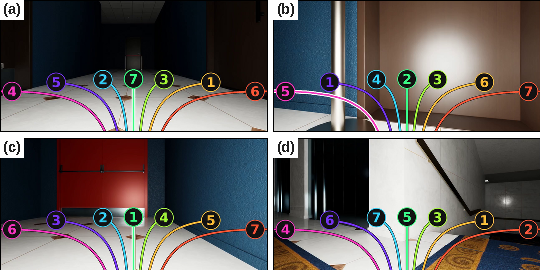
\includegraphics{figures/fig4_qualitative.pdf}
\Description{Four camera frames with seven coloured arcs and shuffled number labels drawn on the
floor. (a) An open hallway with a door far ahead. (b) A wall and a metal pole close ahead, with
open floor to the far left. (c) A red emergency exit door straight ahead. (d) An elevator lobby
with a wall and dark doorframe ahead and carpet in the foreground.}
\caption{Two successful runs, text quoted from the logs. (a--c)~``Go straight ahead through
the hallway, then turn left at the end to approach the red emergency exit door.'' (a)~``The
way ahead is open\ldots TARGET: not visible'' $\rightarrow$ straight at 0.45\,m/s. (b)~``A
wall straight ahead\ldots most open floor is to the far left'' $\rightarrow$ $\kappa=+0.60$.
(c)~``A red double door\ldots TARGET: 3\,m'' $\rightarrow$ straight at a model-chosen
0.20\,m/s. (d)~``\ldots stop at the nearest elevator.'' ``A wall and a dark doorframe
ahead\ldots TARGET: not visible'' $\rightarrow$ STOP, meaning \emph{blocked}; a balk
recovery forced a new decision.}
\label{fig:qual}
\end{figure}

In Fig.~\ref{fig:qual}a--c the select call follows the description's direction word and the
TARGET line sets the speed. Panel (d) is the most frequent failure in our development runs,
\emph{STOP-means-blocked}: in one elevator run the model answered STOP on 42 of 65 decisions
from 5.5\,m out while its description named an open side; STOP should be gated on a
visible, near target. Runs also
\emph{arrive and leave}, passing within 2.2\,m of the goal and driving on, and in the 34\,m
open warehouse, straight on 210 of 222 non-STOP decisions with a small right bias integrated
into an orbit of $-506^\circ$ cumulative yaw. Underneath, the select call is close to a lookup
on the description's direction word: over 840 decisions ``straight'' led to the straight arc
94\% of the time, and with the word fixed the correlation between goal bearing and chosen
curvature was only 0.04--0.11. The target was ``not visible'' on 65\% of decisions, rising
from 42\% to 92\% with the turn an episode requires. QVLA obeys explicit directions and avoids
obstacles but does not search for a goal it cannot see, which is where it lost to TIC-VLA
(Sect.~\ref{sec:closed}).

\section{Limitations and Conclusion}
\label{sec:conclusion}

All results are simulated, on one robot with a kinematic base and a contact layer, over 13
indoor episodes chosen from those TIC-VLA completes on its own robot, three runs each. A 27B
model needs a dedicated 32\,GB GPU and about 2.1\,s per decision, which the asynchronous plan
hides only while the scene changes slowly. Within these limits, a frozen VLM that may only
choose among paths drawn in its own image follows instructions far more than a navigation VLA
fine-tuned for the task (102$^\circ$ against at most 36$^\circ$) and, without any training,
reaches a similar number of goals (7.7 against 6.3 of 13, not significant). This rests on
two cheap choices: shuffled labels on arcs that are the controller's own plans, and a first
call that names the open side. Its failures show what is missing, a search for goals it
cannot yet see; that, and a physical robot, are next.

\begin{credits}
\subsubsection{\ackname}
This work has been supported by the Research Fund of Gebze Technical University. Project
Number: 2026-A-113-27.

\subsubsection{\discintname}
The authors have no competing interests to declare that are relevant to the content of this
article.
\end{credits}
%
\bibliographystyle{splncs04}
\bibliography{references}
%
\end{document}
